\chapter{Exploration}\label{chap:expl}

This chapter will go over the exploratory part of this work, discussing
experiments and analyses that were done in order to understand the functionality
of eBPF and how the network stack and mac80211 subsystem in the Linux kernel
work.


\section{Analysis of the mac80211 Subsystem}\label{sect:mac802}

The general idea for the tool that was to be developed was something that would
record the activity of a network and then display the changes that happened in
that network in a timeline. Alongside those events, we would have the packets
that caused them, so that the user could inspect those packets. But we still
needed to get to grips with eBPF because we had no prior experience with it.


\subsection{Exploration of the Network Stack}

We decided to begin by analysing the Linux source code using the Elixir Cross
Referencer~\cite{elixir}, and wrote small scripts with \textbf{bpftrace} to
better understand how the many components of eBPF, like maps and probes, could
be used to accomplish our objective, as well as to find the limits of this
technology. An example of one of these scripts was one that calculated the time
it took to send a \ac{UDP} network packet via the \texttt{sendto} system call
until the data to be transmitted reached the network card.

We started by seeing how glibc (GNU C Library) version 2.34 called the
\texttt{sendto} system call of the Linux kernel (version 5.15), and from there
followed the function calls in the kernel's code until we reached the function
\texttt{\_\_netdev\_start\_xmit}, which sends the data to be transmitted to the
appropriate network driver. This part was somewhat difficult, as most functions
could diverge, and macros are used a lot. The path of functions we followed for
IPv4 \ac{UDP} packets can be seen in \autoref{fig:callstack}.

\begin{figure}[htb]
   \centering
   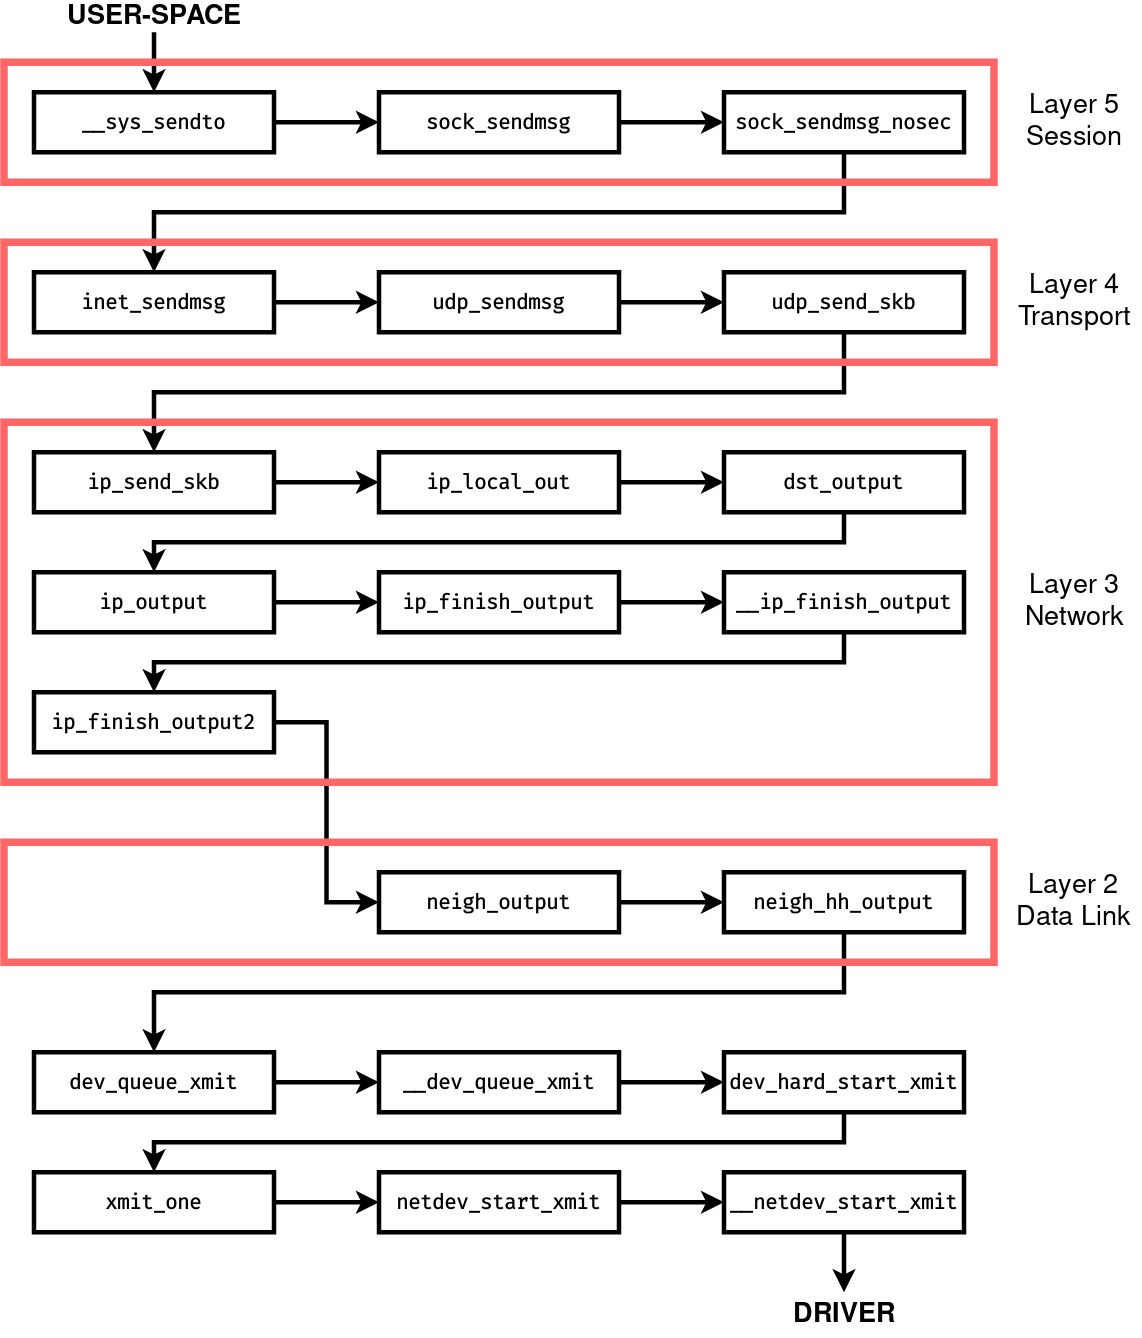
\includegraphics[scale=.375]{callstack2}
   \caption{Call stack analysed for packet transmission}\label{fig:callstack}
\end{figure}

For the script to record the time taken, we decided to use the entry tracepoint
of the \texttt{sendto} system call to save the timestamp of the call, and put a
probe in \texttt{\_\_netdev\_start\_xmit} to calculate the time taken. However,
we ran into an error because this function is inlined, and thus can not be
probed. The last function that can be probed is \texttt{dev\_hard\_start\_xmit},
but we could also probe the exit tracepoint of the \texttt{sendto} system call.
We decided to probe both the function and the exit tracepoint, for both to
calculate the time. This way we would get two different times: the time it took
from the system call until it reached the \texttt{dev\_hard\_start\_xmit}
function, and the time it took for the whole system call to complete. The code
for this script can be seen in \autoref{app:timer}.


\subsection{Use of Emulation}

We wanted to monitor \ac{IEEE} 802.11s mesh networks in particular, and to
perform tests we would need a mesh network. For this, we opted to go with an
emulated network instead of using real hardware to save on time and to make
testing simpler and more predictable (ability to remove interference, adjustable
antenna range, etc.). We used Mininet-WiFi~\cite{mnwifi}, which had everything
we needed, and even included the setup for an example mesh network.

We quickly ran into an issue with Mininet-WiFi, however. The Linux distribution
we were using to develop our tool (Arch Linux) was not officially supported by
Mininet-WiFi. Thankfully, the network emulator had virtual machine images
available for this type of situation, but we had some trouble with the packages
in the repositories of the distribution used by the virtual machine. Not only
was the version of \textbf{bpftrace} available quite old, but the package of the
kernel headers provided, which were used to get structure definitions, only had
the files from the \textbf{include} directory of the kernel source code,
contrary to the distribution we were using, which had all header files. These
issues were preventing some of our scripts from running. To solve this, we
decided to try to install Mininet-WiFi manually in our system, despite it using
a distribution that was not officially supported. Although it required some
manual dependency checking and installing, the Mininet-WiFi installation worked
without problems.


\subsection{Finding Relevant Mesh Network Functions}\label{subs:mesh}

Because our focus was on \ac{IEEE} 802.11s mesh networks, we decided to check
the content of the mac80211 subsystem. We tried to find resources that mentioned
which functions were used to manipulate the system's mesh path table, but all we
found were links to the source code files, which we already had. The only
solution that seemed viable was to find these functions ourselves. Using version
5.10 of the Linux kernel, we started by going through all the files that had
``mesh'' in their name in the mac80211 subsystem folder, saving the names of all
of their functions. We then wrote a basic \textbf{bpftrace} script that probed
all of these functions, printing their names if they were called. This way,
whenever something that had to do with mesh networking happened in the kernel,
we would see the names of the functions that were executed. This script was
quite big, but a snippet of it can be found in \autoref{app:calls}.

With Mininet-WiFi up and running a simple \ac{IEEE} 802.11s mesh network
composed of 3 stations, where 2 stations were too far apart to communicate
directly (station 1 and station 3) and had to use the third one (station 2) as a
``bridge'' to communicate, we executed the script we wrote for around 10 seconds
and pinged station 3 from station 1. We noticed in the output that a lot of
functions were showing up, and by analysing the content of these functions, as
well as their comments (if they had any), we realised that most of them could be
ignored, as they performed actions that did not affect the mesh path table.
After removing the functions that are not relevant for monitoring path changes,
we ended up with two functions in our list: \texttt{mesh\_path\_add}, which
inserts a mesh path in the mesh path table, and
\texttt{mesh\_path\_assign\_nexthop}, which changes the \textbf{nexthop} value
of a given mesh path. We didn't see any paths being deleted, which was expected
given that the test performed was short. However, knowing that the deletion of
paths was possible, we considered \texttt{mesh\_path\_del} as well.


\subsection{Choice of eBPF Framework}

With these functions in mind, we started developing our program. We had to make
a choice between using \ac{BCC} or \ac{CO-RE}. Although more complex and with
less documentation, we decided to try \ac{CO-RE}, using the libbpf-bootstrap
repository available. However, we quickly hit a wall. The example in the blog
posts made by the author of \ac{CO-RE} mentioned that the file containing the
structure and type definitions used in the kernel needed to be generated with
the \texttt{bpftool} command, using the \ac{BTF} file
\texttt{/sys/kernel/btf/vmlinux}. The command seemed to have worked at first,
but including the generated file in our program was resulting in the error of
unknown structures used. Not finding any mention of this issue anywhere, and
with all the examples available using the exact the same command, we decided to
switch to \ac{BCC} using Python. Because the kernel headers package provided by
the distribution we were using included all the header files of the Linux source
code, we had no problems of unknown structures using \ac{BCC}.


\subsection{Probing Packet Transmission and Reception}\label{subs:pkt}

The idea of our program was to retrieve the data of the mesh path that was
inserted, modified, or removed from a mesh path table, by probing the functions
that performed these actions when a thread executed them, store that data in a
BPF map, and when that same thread passed through the tracepoint at packet
transmission/reception, load the data stored in the BPF map, add the data link
layer of the packet detected at the tracepoint to it, and send it to user-space
to be processed by the user-space portion of the program. We had already found
the functions used to retrieve the details of paths that were involved in
modifications performed in the mesh path table, but we still needed a way to get
the content of the packets that caused these actions. Thanks to the previously
mentioned test that was done at the beginning with bpftrace, we found a couple
of tracepoints inside the \texttt{xmit\_one} function that provided access to
the \texttt{sk\_buff} structure that holds the contents of packets.

For packet reception however, the task was a bit harder. We found a tracepoint
that worked, but the issue was that, because we are dealing with packet
reception, this tracepoint is called before any calls to functions that modify
the mesh path table, and we need to delete the content that was stored in the
BPF map for threads that did not change the mesh path table so as not to cause
memory leaks. This issue can be visualised in the difference between
\autoref{fig:pkttx} and \autoref{fig:pktrx}, where every thread that deals with
packet reception stores data in the BPF map, but only the ones that deal with
mesh paths delete the content stored when it is no longer needed, leaving the
contents stored by the other threads in the BPF map, with no way of deleting
them.

One way to solve this issue would be to find another tracepoint or function to
probe located after any change to the mesh path table, to capture all executions
that also passed through the packet reception tracepoint in order to delete the
content stored in the BPF map that was not used. Unfortunately, we did not find
any tracepoint of function we could probe that met these requirements.

\begin{figure}[htb]
   \centering
   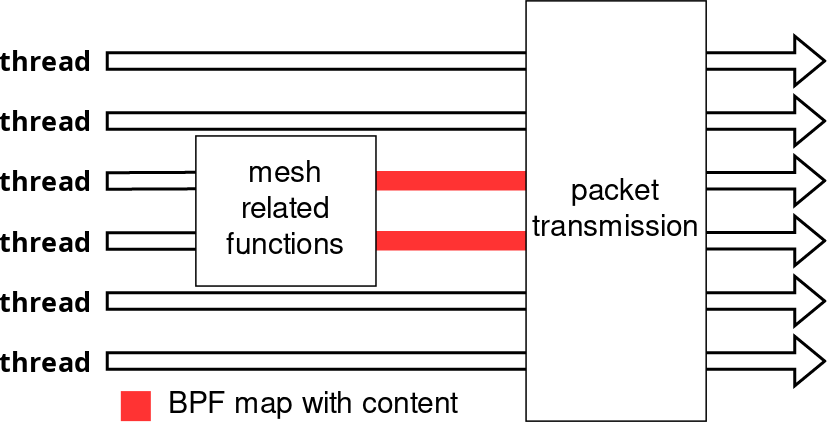
\includegraphics[scale=.4]{pktout}
   \caption{Use of BPF maps in packet transmission}\label{fig:pkttx}
\end{figure}

\begin{figure}[htb]
   \centering
   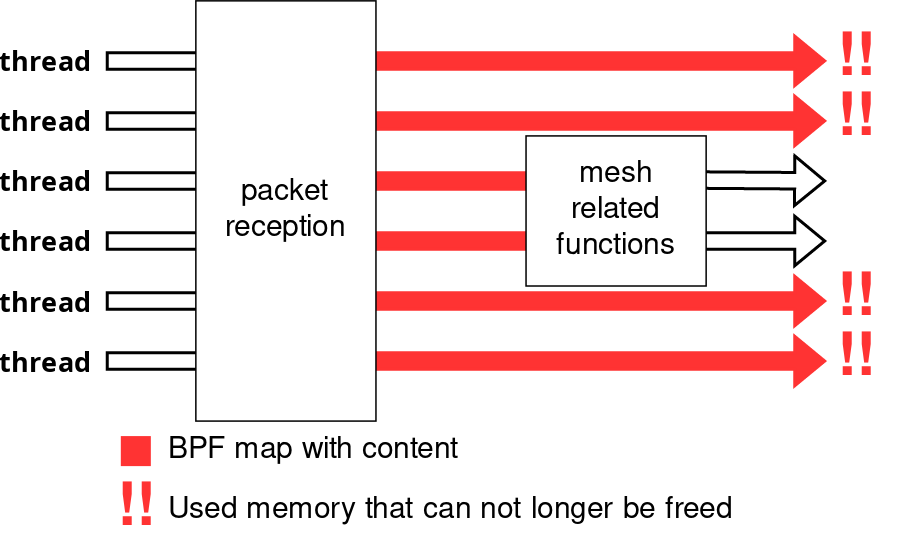
\includegraphics[scale=.4]{pktin}
   \caption{use of BPF maps in packet reception}\label{fig:pktrx}
\end{figure}

Because of this, we had to look for an alternative. We wrote a one-line script,
shown in \autoref{scr:stack}, that printed the call stack of kernel threads when
they passed through \texttt{mesh\_path\_add}, and found that the function
\texttt{ieee80211\_mesh\_rx\_queued\_mgmt} was called every time (except for
when mesh paths were added by packet transmission instead of reception), and it
had the \texttt{sk\_buff} structure in its arguments. After checking that this
function was called by a worker thread that executed
\texttt{ieee80211\_iface\_process\_skb} for every packet received, we decided to
use \texttt{ieee80211\_mesh\_rx\_queued\_mgmt}. We would still need to use two
probes, one at the function entry and another at the exit (because \ac{BCC}
can't get function arguments at the exit), but we could ensure that everything
that was written into the BPF map would later be removed.

\begin{sloppypar}
While looking for solutions to this problem, we also stumbled upon some
tracepoints that are called on commands from user-space that affected the mesh
path table, including insertion, modification, and deletion of mesh paths,
through the usage of the functions \texttt{ieee80211\_add\_mpath},
\texttt{ieee80211\_change\_mpath}, and \texttt{ieee80211\_del\_mpath}
respectively. Along with these tracepoints, there are also tracepoints at the
exit of these actions, used to retrieve the exit value of these functions.
Because these three functions all return \texttt{int}, we decided to add the
tracepoint \texttt{rdev\_return\_int} to our program to capture actions that
modify the mesh path table taken from the user-space.
\end{sloppypar}

\lstinputlisting[caption={Script to print the kernel stack},label=scr:stack,float=hb]{kstack.bpf}


\subsection{Capturing Relevant Packets}

At this point, we had the structure of the eBPF program pretty much set, but
there was still one thing we wanted to improve. We had access to the packets,
but we did not want to send their whole content to user-space, since we only
needed the content of the data link layer. While looking around the Linux
kernel, searching for how to access the fields that we would need, we found the
structure \texttt{ieee80211\_hdr} in the file
\texttt{include/linux/ieee80211.h}, and in the same file we found some functions
that led to examples of how the structure could be used, which was to cast the
\texttt{data} field of the \texttt{sk\_buff} as an \texttt{ieee80211\_hdr}
structure pointer.

We wrote a script that had a probe in the function \texttt{mesh\_path\_add}
where it added its thread ID in an BPF map, using the thread ID as the key as
well, and in the tracepoint \texttt{net:net\_dev\_xmit}, used in packet
transmission, it cast the \texttt{data} field of the \texttt{sk\_buff} structure
as an \texttt{ieee80211\_hdr} and printed all of its fields, if and only if the
BPF map had its thread ID stored. This resulted in the script printing the link
layer of packets that were being sent by threads that had inserted a mesh path
to the mesh path table earlier.

Running this script, we found that all the fields were correct except for the
address 1 field, which identifies the immediate receiver of the frame. Instead
of the address that was shown in the corresponding packet in Wireshark, the
field showed up as all zeros. After a bit of thinking, we realised that this
address shows as all zeros because the system that sent this packet only knew
the destination, but not the receiver, which could be the destination itself, or
any other device. Because this field would cause problems when comparing with
packets from the packet capture files, we decided to ignore addresses that show
as all zeros.


\subsection{Switch from BCC to CO-RE}\label{subs:switch}

After making sure the program worked in the emulated environment, it was time to
test it with real hardware. We started with a couple of computers with different
distributions (one with Arch Linux and another with Fedora) and a Raspberry Pi.
However, we ran into an issue we had already faced before. Just like the
distribution used by the Mininet-WiFi virtual machine, most distributions'
kernel header packages only include the header files present in the
\textbf{include} directory of the Linux source code, meaning that some of the
structures we were using were not available in the Raspberry Pi, Ubuntu, Fedora,
etc. We could solve this by copying the structures we needed to our program, but
these structures have other structures as fields, which meant we needed to copy
even more structures. Not only that, but we would also need to be cautious of
Linux updates changing the contents of these structures. Another option would be
to make the program depend on the Linux source code, but not all distributions
provide the source code as a package, and this would also need to be updated
along with the kernel itself. We ended up trying to see if we could go back to
using \ac{CO-RE}. After some time, we found that \texttt{vmlinux} was not the
only file in the \texttt{/sys/kernel/btf/} folder. It includes plenty more
files, one of them named \texttt{mac80211}. We tried generating the file with
the structure and type definitions using \texttt{/sys/kernel/btf/mac80211}, and
testing it, it worked without issues. As a result, we decided to switch
completely to \ac{CO-RE}.

We would need to switch from Python as we did not find a wrapper for it for
libbpf, which is needed to use \ac{CO-RE}. The languages we could use were
C/C++, Rust, or Go. We didn't want to deal with manual memory management if we
could, and with very little Go experience, so we decided to use Rust. Because of
how \ac{CO-RE} works, the eBPF portion also required some changes. One of the
biggest changes was the removal of the entry probe for
\texttt{ieee80211\_mesh\_rx\_queued\_mgmt}, because, unlike \ac{BCC}, \ac{CO-RE}
can access the arguments of a function at its exit. However, because arguments
can be pointers, as is the case for the argument with the packet content, the
content they point to at the exit can be different from the content they pointed
to at the entry. We did a few tests to check if the content of the packet
changed during the execution of the function and found that it never happened.
In the future, a more thorough assessment will be necessary to make sure that
this is always the case. Because using a single probe at the exit would simplify
the code structure, and we never saw the content of the packet change, we
decided to remove the probe at the beginning. The other main change was the
switch from probing \texttt{mesh\_path\_del} to \texttt{\_\_mesh\_path\_del}. We
did this because we were unable to retrieve the destination field of the path
from the arguments of \texttt{mesh\_path\_del}. We believe \ac{CO-RE} is capable
of this, but none of the examples provided helped in finding a solution. When
modifying the probe, we noticed that \texttt{\_\_mesh\_path\_del} was called
from other parts of the code as well, not just \texttt{mesh\_path\_del}, so we
added a few more probes to take those calls into consideration. These are
explained in detail in \autoref{subsec:ebpfcode}.

With these changes in place, the program started working on all the
distributions we were testing, but it still was not working in the Raspberry Pi.
Using the command \texttt{zgrep BTF /proc/config.gz}, we found that the kernel
being used in the Raspberry Pi was not built with \ac{BTF} support. Most
distributions build the kernel with this support for the x86 architecture, but
none of the distributions we tried for the Raspberry Pi offered the kernel with
\ac{BTF} support compiled in, so we tried to compile the kernel ourselves.
Unfortunately, that also failed without us understanding why. To prevent this
issue from blocking our progress, we decided to continue the development leaving
the Raspberry Pi aside for a later date.


\section{Event Capture and Packet Association}\label{sect:evepktasc}

As the main objective of the program was to show the user details about paths
that were added, modified, or removed from a system's mesh path table, along
with the respective packet that caused that action, we had to obtain this
information somehow.

Getting the details of paths was the easy part. As mentioned above, we probed
the functions that modified the mesh path table, and since they have a pointer
to the path structure in their arguments (except for \texttt{mesh\_path\_add}
which has other structures), we could take the information directly and store it
in a BPF map to send it to the user-space later.

The work required to get the packet content was somewhat more involved. In the
tests that we performed earlier, we noticed that whenever the mesh path table
was modified, functions related to packet transmission or reception were
executed, which meant that we could get the packet that caused the action by
following the thread's path. We set the probe and tracepoint used for packet
reception and transmission respectively mentioned earlier, and used the thread's
ID to check if a thread that was receiving/transmitting a packet had passed
through a function that modified the mesh path table earlier, and, if it did,
use that packet's content. Instead of sending the whole packet to the
user-space, we used a structure called \texttt{ieee80211\_hdr} to get just the
elements we needed in order to be able to unambiguously identify the packet.
We do this to keep the memory usage as low as possible and to minimise the
overhead of our eBPF programs. The fields we take from the packet are the
\textbf{Frame Control}, \textbf{Sequence Control}, and \textbf{QoS Control}
(when available) fields, as well as the three (four in some cases) MAC
addresses. We use the \textbf{Frame Control} to check the size of the data link
layer, as well as to check if the \textbf{QoS Control} field is included and if
there are three or four addresses. The \textbf{Sequence Control} is used to
differentiate packets that have all the other fields equal. According to section
10.3.2.14 of the \ac{IEEE} 802.11 standard~\cite{ieee80211}, only the first two
addresses of the MAC layer are needed to identify packets, along with the
\textbf{QoS Control} field, when it is present. Because we already had the
\textbf{Frame Control}, we thought we might as well use it for packet comparison
as well. We ended up not using the third and fourth addresses, but kept them as
well in case they would be needed in the future.
